%package list
\documentclass{article}
\usepackage[top=3cm, bottom=3cm, outer=3cm, inner=3cm]{geometry}
\usepackage{multicol}
\usepackage{graphicx}
\usepackage{url}
%\usepackage{cite}
\usepackage{hyperref}
\usepackage{array}
%\usepackage{multicol}
\newcolumntype{x}[1]{>{\centering\arraybackslash\hspace{0pt}}p{#1}}
\usepackage{natbib}
\usepackage{pdfpages}
\usepackage{multirow}
\usepackage[normalem]{ulem}
\useunder{\uline}{\ul}{}
\usepackage{svg}
\usepackage{xcolor}
\usepackage{listings}

\lstdefinestyle{ascii-tree}{
    literate={├}{|}1 {─}{--}1 {└}{+}1 
  }
\lstset{basicstyle=\ttfamily,
  showstringspaces=false,
  commentstyle=\color{red},
  keywordstyle=\color{blue}
}
%\usepackage{booktabs}
\usepackage{caption}
\usepackage{subcaption}
\usepackage{float}
\usepackage{array}

\newcolumntype{M}[1]{>{\centering\arraybackslash}m{#1}}
\newcolumntype{N}{@{}m{0pt}@{}}


%%%%%%%%%%%%%%%%%%%%%%%%%%%%%%%%%%%%%%%%%%%%%%%%%%%%%%%%%%%%%%%%%%%%%%%%%%%%
%%%%%%%%%%%%%%%%%%%%%%%%%%%%%%%%%%%%%%%%%%%%%%%%%%%%%%%%%%%%%%%%%%%%%%%%%%%%
\newcommand{\itemEmail}{aphoccot@unsa.edu.pe}
\newcommand{\itemStudent}{Alejandro Josue Phocco Tapia}
\newcommand{\itemCourse}{Programación Web 2}
\newcommand{\itemCourseCode}{20220589}
\newcommand{\itemSemester}{III}
\newcommand{\itemUniversity}{Universidad Nacional de San Agustín de Arequipa}
\newcommand{\itemFaculty}{Facultad de Ingeniería de Producción y Servicios}
\newcommand{\itemDepartment}{Departamento Académico de Ingeniería de Sistemas e Informática}
\newcommand{\itemSchool}{Escuela Profesional de Ingeniería de Sistemas}
\newcommand{\itemAcademic}{2023 - A}
\newcommand{\itemInput}{Del 14 Junio 2023}
\newcommand{\itemOutput}{\today}
\newcommand{\itemPracticeNumber}{06}
\newcommand{\itemTheme}{Python - Django}
%%%%%%%%%%%%%%%%%%%%%%%%%%%%%%%%%%%%%%%%%%%%%%%%%%%%%%%%%%%%%%%%%%%%%%%%%%%%
%%%%%%%%%%%%%%%%%%%%%%%%%%%%%%%%%%%%%%%%%%%%%%%%%%%%%%%%%%%%%%%%%%%%%%%%%%%%

\usepackage[english,spanish]{babel}
\usepackage[utf8]{inputenc}
\AtBeginDocument{\selectlanguage{spanish}}
\renewcommand{\figurename}{Figura}
\renewcommand{\refname}{Referencias}
\renewcommand{\tablename}{Tabla} %esto no funciona cuando se usa babel
\AtBeginDocument{%
	\renewcommand\tablename{Tabla}
}

\usepackage{fancyhdr}
\pagestyle{fancy}
\fancyhf{}
\setlength{\headheight}{30pt}
\renewcommand{\headrulewidth}{1pt}
\renewcommand{\footrulewidth}{1pt}
\fancyhead[L]{\raisebox{-0.2\height}{
\includegraphics[width=3cm]{img/logo_episunsa.png}}}
\fancyhead[C]{\fontsize{7}{7}\selectfont	\itemUniversity \\ \itemFaculty \\ \itemDepartment \\ \itemSchool \\ \textbf{\itemCourse}}
\fancyhead[R]{\raisebox{-0.2\height}{
\includegraphics[width=1.2cm]{img/logo_abet}}}
\fancyfoot[L]{Estudiante Alejandro Phocco Tapia}
\fancyfoot[C]{\itemCourse}
\fancyfoot[R]{Página \thepage}

% para el codigo fuente
\usepackage{listings}
\usepackage{color, colortbl}
\definecolor{dkgreen}{rgb}{0,0.6,0}
\definecolor{gray}{rgb}{0.5,0.5,0.5}
\definecolor{mauve}{rgb}{0.58,0,0.82}
\definecolor{codebackground}{rgb}{0.95, 0.95, 0.92}
\definecolor{tablebackground}{rgb}{0.8, 0, 0}

\lstset{frame=tb,
	language=bash,
	aboveskip=3mm,
	belowskip=3mm,
	showstringspaces=false,
	columns=flexible,
	basicstyle={\small\ttfamily},
	numbers=none,
	numberstyle=\tiny\color{gray},
	keywordstyle=\color{blue},
	commentstyle=\color{dkgreen},
	stringstyle=\color{mauve},
	breaklines=true,
	breakatwhitespace=true,
	tabsize=3,
	backgroundcolor= \color{codebackground},
}

\begin{document}

    \vspace*{10px}
	
    \begin{center}	
	\fontsize{17}{17} \textbf{ Informe de Laboratorio \itemPracticeNumber}
    \end{center}
    \centerline{\textbf{\Large Tema: \itemTheme}}
	%\vspace*{0.5cm}	

	\begin{flushright}
		\begin{tabular}{|M{2.5cm}|N|}
			\hline 
			\rowcolor{tablebackground}
			\color{white} \textbf{Nota}  \\
			\hline 
			     \\[30pt]
			\hline 			
		\end{tabular}
	\end{flushright}	

	\begin{table}[H]
		\begin{tabular}{|x{4.7cm}|x{4.8cm}|x{4.8cm}|}
			\hline 
			\rowcolor{tablebackground}
			\color{white} \textbf{Estudiante} & \color{white}\textbf{Escuela}  & \color{white}\textbf{Asignatura}   \\
			\hline 
			{\itemStudent \par \itemEmail} & \itemSchool & {\itemCourse \par Semestre: \itemSemester \par Código: \itemCourseCode}     \\
			\hline 			
		\end{tabular}
	\end{table}		
	
	\begin{table}[H]
		\begin{tabular}{|x{4.7cm}|x{4.8cm}|x{4.8cm}|}
			\hline 
			\rowcolor{tablebackground}
			\color{white}\textbf{Laboratorio} & \color{white}\textbf{Tema}  & \color{white}\textbf{Duración}   \\
			\hline 
			\itemPracticeNumber & \itemTheme & 04 horas   \\
			\hline 
		\end{tabular}
	\end{table}
	
	\begin{table}[H]
		\begin{tabular}{|x{4.7cm}|x{4.8cm}|x{4.8cm}|}
			\hline 
			\rowcolor{tablebackground}
			\color{white}\textbf{Semestre académico} & \color{white}\textbf{Fecha de inicio}  & \color{white}\textbf{Fecha de entrega}   \\
			\hline 
			\itemAcademic & \itemInput &  \itemOutput  \\
			\hline 
		\end{tabular}
	\end{table}
	
    \section{Tarea}
	\begin{itemize}		
		\item Crearemos una pagina de viajes, usando un video como base: \url{https://www.youtube.com/watch?v=OTmQOjsl0eg}
            \begin{figure}[H]
    		\centering
    		
\includegraphics[width=0.25\textwidth,keepaspectratio]{img/django.png}
    	\end{figure}
	\end{itemize}

	
    \section{URL de Repositorio Github y FLip}
 
        \begin{itemize}
    	\item URL para el laboratorio 06 en el Repositorio GitHub:                                 \url{https://github.com/AlejandroPhoccoTapia/Lab06-PW2-AlejandroPhocco}
            \item URL del video en flip: \url{https://flip.com/s/oX6doXAhZpyQ}
	\end{itemize}
	
    \section{Ejercicios}
 
        \subsection{Estructura del proyecto TravelloApp}
	\begin{itemize}	
	\item Esta es la estructura del proyecto.
	\end{itemize}
	
        \begin{lstlisting}[style=ascii-tree]
        └───TravelloApp
        ├───media
        │   └───pics
        ├───TravelloApp
        │   └───__pycache__
        └───TravelloPeru
            ├───migrations
            │   └───__pycache__
            ├───static
            │   ├───css
            │   └───img
            ├───templates
            └───__pycache__
        \end{lstlisting}  
 
	\subsection{Análisis de archivos }
            
            \begin{itemize}
                \item TravelloApp
            \end{itemize}
    
            \begin{lstlisting}[language=bash,caption={urls.py}][H]
            """
            Django settings for TravelloApp project.
            
            Generated by 'django-admin startproject' using Django 4.2.2.
            
            For more information on this file, see
            https://docs.djangoproject.com/en/4.2/topics/settings/
            
            For the full list of settings and their values, see
            https://docs.djangoproject.com/en/4.2/ref/settings/
            """
            
            from pathlib import Path
            import os
            
            # Build paths inside the project like this: BASE_DIR / 'subdir'.
            BASE_DIR = Path(__file__).resolve().parent.parent
            
            
            # Quick-start development settings - unsuitable for production
            # See https://docs.djangoproject.com/en/4.2/howto/deployment/checklist/
            
            # SECURITY WARNING: keep the secret key used in production secret!
            SECRET_KEY = 'django-insecure-^4&%&dsiofj@dq$e9i(lerp7aexjtm#5$v$r-&%_!l$cjc#9je'
            
            # SECURITY WARNING: don't run with debug turned on in production!
            DEBUG = True
            
            ALLOWED_HOSTS = []
            
            
            # Application definition
            
            INSTALLED_APPS = [
                'django.contrib.admin',
                'django.contrib.auth',
                'django.contrib.contenttypes',
                'django.contrib.sessions',
                'django.contrib.messages',
                'django.contrib.staticfiles',
                'TravelloPeru',
            ]
            
            MIDDLEWARE = [
                'django.middleware.security.SecurityMiddleware',
                'django.contrib.sessions.middleware.SessionMiddleware',
                'django.middleware.common.CommonMiddleware',
                'django.middleware.csrf.CsrfViewMiddleware',
                'django.contrib.auth.middleware.AuthenticationMiddleware',
                'django.contrib.messages.middleware.MessageMiddleware',
                'django.middleware.clickjacking.XFrameOptionsMiddleware',
            ]
            
            ROOT_URLCONF = 'TravelloApp.urls'
            
            TEMPLATES = [
                {
                    'BACKEND': 'django.template.backends.django.DjangoTemplates',
                    'DIRS': [],
                    'APP_DIRS': True,
                    'OPTIONS': {
                        'context_processors': [
                            'django.template.context_processors.debug',
                            'django.template.context_processors.request',
                            'django.contrib.auth.context_processors.auth',
                            'django.contrib.messages.context_processors.messages',
                        ],
                    },
                },
            ]
            
            WSGI_APPLICATION = 'TravelloApp.wsgi.application'
            
            
            # Database
            # https://docs.djangoproject.com/en/4.2/ref/settings/#databases
            
            DATABASES = {
                'default': {
                    'ENGINE': 'django.db.backends.sqlite3',
                    'NAME': BASE_DIR / 'db.sqlite3',
                }
            }
            
            
            # Password validation
            # https://docs.djangoproject.com/en/4.2/ref/settings/#auth-password-validators
            
            AUTH_PASSWORD_VALIDATORS = [
                {
                    'NAME': 'django.contrib.auth.password_validation.UserAttributeSimilarityValidator',
                },
                {
                    'NAME': 'django.contrib.auth.password_validation.MinimumLengthValidator',
                },
                {
                    'NAME': 'django.contrib.auth.password_validation.CommonPasswordValidator',
                },
                {
                    'NAME': 'django.contrib.auth.password_validation.NumericPasswordValidator',
                },
            ]
            
            
            # Internationalization
            # https://docs.djangoproject.com/en/4.2/topics/i18n/
            
            LANGUAGE_CODE = 'en-us'
            
            TIME_ZONE = 'UTC'
            
            USE_I18N = True
            
            USE_TZ = True
            
            
            # Static files (CSS, JavaScript, Images)
            # https://docs.djangoproject.com/en/4.2/howto/static-files/
            
            STATIC_URL = 'static/'
            
            # Default primary key field type
            # https://docs.djangoproject.com/en/4.2/ref/settings/#default-auto-field
            
            DEFAULT_AUTO_FIELD = 'django.db.models.BigAutoField'
            
            MEDIA_URL = '/media/'
            MEDIA_ROOT = os.path.join(BASE_DIR,'media')
    	\end{lstlisting}
     
            Estas son las configuraciones del proyecto. Se debe resaltar el uso de ROOT_MEDIA que servira para guardar las imagenes de los destinos en el proyecto.
        
            \begin{lstlisting}[language=bash,caption={urls.py}][H] 
            from django.contrib import admin
            from django.urls import path, include
            
            urlpatterns = [
                path('admin/', admin.site.urls),
                path('', include('TravelloPeru.urls')),
            ]
            
    	\end{lstlisting}
     
            Estas son las urls del proyectos.

    	\begin{itemize}	
    		\item TravelloPeru
    	\end{itemize}
     
    	\begin{lstlisting}[language=bash,caption={urls.py}][H]
            from django.contrib import admin
            from django.urls import path, include
            from . import views
            from django.conf import settings
            from django.conf.urls.static import static
            
            urlpatterns = [
                path('', views.index, name='index'),
                path('destination/<int:id>', views.destination, name='destination'),
                path('register', views.register, name='register'),
                path('login', views.login, name='login'),
                path('logout', views.logout, name='logout'),
            ]
            
            urlpatterns = urlpatterns + static(settings.MEDIA_URL, document_root=settings.MEDIA_ROOT) 
    	\end{lstlisting}
     
            Estas son las urls utilizadas en la aplicación.

    	\begin{lstlisting}[language=bash,caption={views.py}][H]
            from django.shortcuts import render, redirect
            from .models import Destination
            from django.contrib.auth.models import User, auth
            
            # Create your views here.
            
            def index(request):
                destinations = Destination.objects.all()
            
                return render(request, 'index.html', {'destinations': destinations})
            
            def destination(request, id):
                destination = Destination.objects.get(id=id)
                return render(request, 'destination.html', {'destination': destination})
            
            def register(request):
            
                if request.method == 'POST':
                    first_name = request.POST['first_name']
                    last_name = request.POST['last_name']
                    username = request.POST['username']
                    password = request.POST['password']
                    email = request.POST['email']
            
                    user = User.objects.create_user(username=username, password=password, email=email, first_name=first_name, last_name=last_name)
                    user.save()
            
                    return redirect('/')
                else:
                    return render(request, 'register.html')
            
            def login(request):
                if request.method == "POST":
                    username = request.POST['username']
                    password = request.POST['password']
            
                    user = auth.authenticate(username=username, password=password)
            
                    if user is not None:
                        auth.login(request, user)
                        return redirect('/')
                else:
                    return render(request, 'login.html')
            
            def logout(request):
                auth.logout(request)
                return redirect('/')
    	\end{lstlisting}
     
            Estas son las views utilizadas en la aplicacion.
            
            \begin{lstlisting}[language=bash,caption={Tercera funcion de views.py}][H]
                def logout(request):
                    auth.logout(request)
                    return redirect('/')  
    	\end{lstlisting}
     
            Esta función cierra la sesión del usuario y redirige al usuario a la página principal después de cerrar sesión en la aplicación.

            \begin{lstlisting}[language=bash,caption={models.py}][H]
            from django.db import models
            
            class Destination(models.Model):
                name = models.CharField(max_length=100)
                img = models.ImageField(upload_to="pics")
                desc = models.TextField()
                price = models.IntegerField()
                offer = models.BooleanField(default=False)
            
                def __str__(self):
                    return self.name
    	\end{lstlisting}
     
            Este es el modelo que utilizamos para los destinos.
    

            \begin{itemize}	
    		\item TEMPLATES HTML
    	\end{itemize}
     
    	\begin{lstlisting}[language=bash,caption={nav.html}][H]
            
            
            <!DOCTYPE html>
            <html lang="es">
            <head>
              <meta charset="UTF-8">
              <meta name="viewport" content="width=device-width, initial-scale=1.0">
              <link rel="stylesheet" href="">
            
              <title>Paisajes</title>
            </head>
            <body>
              
              <header class="header">
                <img class="header__img" src="" alt="Icono de la pagina">
                <nav class="nav">
                  <a class="nav__a" href="/">Inicio</a>
            
                  
                  <p class="nav__a">Bienvenido, {{user.first_name}}</p>
                  <a class="nav__a" href="">Cerrar cesión</a>
                  
                  <a class="nav__a" href="">Registrarse</a>
                  <a class="nav__a" href="">Iniciar Sesión</a>
                  
            
                </nav>
              </header>
            
              
            
              
            
              <footer class="footer">
                <p class="footer__p">Alejandro Josue Phocco Tapia</p>
              </footer>
            
            </body>
            </html>
    	\end{lstlisting}
     
            Esta es la plantilla que se reutilizara en las demas. Contiene la barra de navegacion de la pagina.

            \begin{lstlisting}[language=bash,caption={index.html}][H]
            
            
            
            
            
            <main class="main">
            
              <div class="preview">
                <section class="preview__item">
                  <div class="preview__title">
                    <h2 class="preview__h2">Travello Perú</h2>
                  </div>
                  <div class="preview__content">
                    <img src="" alt="paisaje">
                    <p class="preview__p">Perú donde existe un país legendario que posee: fastuosos centros arqueológicos, mágicos sitios naturales y paisajísticos, majestuosos templos precolombinos y coloniales, ancestrales palacios pre-incas e incas, extraordinarios conventos y casonas coloniales, excelentes aguas termo-medicinales, pueblos tradicionales, milenaria cultura, exquisita gastronomía, fina textilería, variada artesanía… y la más grande cultura viva de América.
            
                      Y por si lo anterior fu poco, este mítico país también posee el más grande legado histórico – cultural del Mundo: historia, cultura, gastronomía, aventura, tradición, naturaleza y biodiversidad. Descubre estos lugares.</p>
                  </div>
                </section>
              </div>
            
              <div class="sights">
                <h2 class="sights__h2">Viajes Nacionales</h2>
                <ul class="sights__list">
                  
                  <li class="sights__item">
                    <h3 class="sights__h3">{{destination.name}}</h3>
                    <div class="sights__img-container">
                      
                      <div class="sights__offer">OFERTA</div>
                      
                      <img class="sights__img" src="{{destination.img.url}}" alt="paisaje">
                    </div>
                    <p class="sights__p">price: {{destination.price}}.00$</p>
                    <a class="sights__a" href="/destination/{{destination.id}}">VER</a>
                  </li>
                  
                </ul>
              </div>
            
            </main>
            
            
    	\end{lstlisting}
     
            Esta es la plantilla de la pagina principal de la pagina.

            \begin{lstlisting}[language=bash,caption={destination.html}][H]
            
            
            
              <main class="main">
                <div class="detail">
                  <h2 class="detail__h2">{{destination.name}}</h2>
                  <img class="detail__img" src="{{destination.img.url}}" alt="">
                  <p class="detail__desc">{{destination.desc}}</p>
                  <div class="detail__div">
                    <p class="detail__price">precio: {{destination.price}}.0$</p>
                    
                    <p class="detail__offer">Aprovecha la oferta!!!</p>
                    
                    <button class="detail__button">Comprar</button>
                  </div>
                </div>
              </main>
            
	    \end{lstlisting}
 
            Esta es la plantilla que muestra la informacion de un destino en especifico.

            \begin{lstlisting}[language=bash,caption={login.html}][H]
            
            
            
            <main class="main">
                
              <form class="login" action="login" method="post">
                
                <input class="login__input" type="text" name="username" placeholder="Nombre de Usuario">
                <input class="login__input" type="text" name="password" placeholder="Contraseña">
                <button class="login__button">Ingresar</button>
              </form>
            
            </main>
            
	\end{lstlisting}
 
            Esta es la plantilla para la pagina de ingreso.

            \begin{lstlisting}[language=bash,caption={register.html}][H]
            
            
            
              <main class="main">
                
                <form class="register" action="register" method="post">
                  
                  <input class="register__input" type="text" name="first_name" placeholder="Nombre">
                  <input class="register__input" type="text" name="last_name" placeholder="Apellido">
                  <input class="register__input" type="text" name="username" placeholder="Nombre de Usuario">
                  <input class="register__input" type="email" name="email" placeholder="Email">
                  <input class="register__input" type="text" name="password" placeholder="Contraseña">
                  <button class="register__button">Registrarse</button>
                </form>
            
              </main>
            
	\end{lstlisting}
 
            Esta es la plantilla para la registracion de un usuario.

            \begin{itemize}
                \item Accediendo a css/index.css
            \end{itemize}
            
            \begin{lstlisting}[language=bash,caption={index.css}][H]
            body {
              min-height: 100vh;
              padding: 0;
              margin: 0;
              display: flex;
              flex-direction: column;
            }
            
            .header {
              height: 3rem;
              background-image: linear-gradient(to top, hsl(120 90% 30%), hsl(120 80% 20%));
              padding: 1rem;
              display: flex;
              flex-direction: row;
              justify-content: space-between;
              align-items: center;
            }
            
            .header__img {
              width: 5rem;
              box-sizing: border-box;
            }
            
            .nav {
              height: 100%;
              display: flex;
              gap: 2rem;
              flex-direction: row;
              justify-content: space-evenly;
              align-items: center;
            }
            
            .nav__a {
              text-decoration: none;
              display: inline-block;
              background-color: hsl(0 100% 100%);
              padding: 0.25rem 0.75rem;
              font-weight: bolder;
              font-size: 1.25rem;
              border-radius: 1rem;
              transition: background-color 100ms, color 100ms;
            }
            
            .nav__a:hover {
              background-color: hsl(0 0% 0%);
              color: hsl(0 100% 100%);
            }
            
            .main {
              background-image: linear-gradient(to left bottom, hsl(0 100% 100%), hsl(0 0% 50%));
              height: 100%;
              flex-grow: 1;
              display: flex;
              flex-direction: column;
              align-items: center;
              justify-content: space-around;
              padding: 1.5rem;
              gap: 2rem;
            }
            
            .preview {
              display: flex;
              width: 100%;
              flex-direction: column;
              gap: 1.5rem;
            }
            
            .preview__item {}
            
            .preview__title {
              display: flex;
              justify-content: center;
              align-items: center;
              background-color: hsl(0 0% 40%);
              padding: 0.5rem;
              border-radius: 01rem;
              margin: 0 0 1rem 0;
            }
            
            .preview__h2 {
              color: hsl(0 100% 100%);
              margin: 0;
            }
            
            .preview__content {
              background-color: hsl(0 100% 100%);
              display: flex;
              gap: 1rem;
              padding: 1rem;
              border-radius: 1rem;
              box-shadow: 0 5px 10px 5px;
            }
            
            .preview__img {
              flex-basis: 40%;
            }
            
            .preview__p {
              flex-basis: 60%;
              font-size: 1.5rem;
            }
            
            .sights {
              background-color: hsl(0 100% 100%);
              display: flex;
              flex-direction: column;
              align-items: center;
              width: 100%;
              border-radius: 1rem;
              box-shadow: 0 5px 10px 5px;
            }
            
            .sights__h2 {
              display: flex;
              justify-content: center;
              align-items: center;
              color: hsl(0 100% 100%);
              background-color: hsl(0 0% 40%);
              padding: 0.5rem;
              border-radius: 1rem;
              width: 100%;
              margin: 0 0 1rem 0;
              box-sizing: border-box;
            }
            
            .sights__list {
              box-sizing: border-box;
              list-style: none;
              margin: 0;
              padding: 1rem;
              width: 75%;
              display: grid;
              grid-template-columns: repeat(auto-fit, minmax(300px, 1fr));
              justify-content: center;
              gap: 2rem;
            }
            
            .sights__item {
              background-color: hsl(0 0% 100%);
              background-image: linear-gradient(to left bottom, hsl(0 0% 100%), hsl(180 100% 45%), hsl(240 100% 55%));
              border: 0.25rem solid hsl(0 0% 30%);
              border-radius: 0.5rem;
              display: flex;
              flex-direction: column;
              align-items: center;
              position: relative;
              padding: 0.75rem 0;
              transition: transform 150ms;
              overflow: hidden;
            }
            
            .sights__item:hover {
              transform: scale(1.1);
            }
            
            
            .sights__h3 {
              margin: 0 0 0.5rem 0;
              font-size: 1.375rem;
            }
            
            .sights__img-container {
              box-sizing: content-box;
              position: relative;
            }
            
            .sights__offer {
              position: absolute;
              z-index: 1;
              background-color: red;
              right: 5%;
              top: 5%;
              display: inline-block;
              padding: 0.25rem;
              border-radius: 0.5rem;
              color: hsl(0 0% 100%)
            }
            
            .sights__img {
              margin: 0 0 0.5rem 0;
              height: 10rem;
            }
            
            .sights__p {
              margin: 0;
              margin: 0 0 0.25rem 0;
              padding: 0.25rem 0.5rem;
              background-color: hsl(0 100% 100%);
              border-radius: 0.25rem;
              color: hsl(120 100% 35%)
            }
            
            .sights__a {
              text-decoration: none;
              display: inline-block;
              padding: 0.125rem 0.5rem;
              margin: 0;
              background-color: hsl(120, 80%, 32%);
              color: hsl(30 0% 100%);
              border: 2px solid hsl(0 0% 0%);
              border-radius: 0.25rem;
            }
            
            .sights__a:hover {
              background-color: hsl(0 0% 0%);
              border: 2px solid hsl(0 0% 0%);
            }
            
            .footer {
              display: flex;
              justify-content: center;
              align-items: center;
              background-color: hsl(0 0% 25%);
            }
            
            .footer__p {
              color: hsl(0 100% 100%);
            }
            
            .detail {
              background-color: hsl(0 100% 100%);
              border-radius: 2rem;
              display: flex;
              flex-direction: column;
              align-items: center;
              width: min(40rem, 90vw);
              padding: 1rem 2rem;
              overflow: hidden;
            }
            
            .detail__h2 {
              font-size: 2rem;
              margin: 0 0 1rem 0;
            }
            
            .detail__img {
              height: 20rem;
              margin: 0 0 2rem 0;
            }
            
            .detail__desc {
              margin: 0 0 1rem 0;
            }
            
            .detail__div {
              width: 100%;
              height: 5rem;
              display: flex;
              justify-content: space-between;
              align-items: center;
            }
            
            .detail__price {
              display: inline-block;
              background-color: green;
              padding: 0.5rem;
              border-radius: 0.25rem;
              color: white;
            }
            
            .detail__offer {
              display: inline-block;
              background-color: red;
              padding: 0.5rem;
              border-radius: 0.25rem;
              color: white;
            }
            
            .detail__button {
              background-color: orange;
              border: none;
              color: white;
              font-size: 1.125rem;
              padding: 0.5rem 1.5rem;
              border-radius: 1rem;
              cursor: pointer;
            }
            
            .detail__button:hover {
              background-color: white;
              color: orange;
              border: 1px solid hsl(0 0% 0%);
            }
            
            .register {
              background-color: hsl(0 100% 100%);
              border-radius: 2rem;
              box-shadow: 0 5px 30px 5px hsl(0 0% 40%);
              display: flex;
              flex-direction: column;
              align-items: center;
              gap: 1rem;
              padding: 2rem;
            }
            
            .register__input {
              height: 1.5rem;
              width: 15rem;
            }
            
            .register__button {
              padding: 0.5rem 2rem;
              background-color: hsl(240 100% 45%);
              border: none;
              color: hsl(0 100% 100%);
              border-radius: 0.5rem;
            }
            
            .register__button:hover {
              background-color: hsl(0 100% 100%);
              border: 1px solid hsl(0 0% 0%);
              color: hsl(240 100% 45%);
            }
            
            
            .login {
              background-color: hsl(0 100% 100%);
              border-radius: 2rem;
              box-shadow: 0 5px 30px 5px hsl(0 0% 40%);
              display: flex;
              flex-direction: column;
              justify-content: center;
              align-items: center;
              padding: 2rem;
              gap: 1rem;
            }
            
            .login__input {
              height: 1.5rem;
              width: 15rem;
              margin: 0;
            }
            
            .login__button {
              padding: 0.5rem 2rem;
              background-color: hsl(240 100% 45%);
              border: none;
              color: hsl(0 100% 100%);
              border-radius: 0.5rem;
            }
            
            .login__button:hover {
              background-color: hsl(0 100% 100%);
              border: 1px solid hsl(0 0% 0%);
              color: hsl(240 100% 45%);
            }
	\end{lstlisting}
 
            Este es el archivo css que le da estilo a toda la pagina se uso la metodologia BEM para el nombramiento de las clases.
        
        \subsection{Demostracion de pagina}
            \textbf{Ahora veremos como se ve la pagina:}\\
            
            Primero iniciaremos el servidor y veremos la pantalla inicial:
            \\ \\
            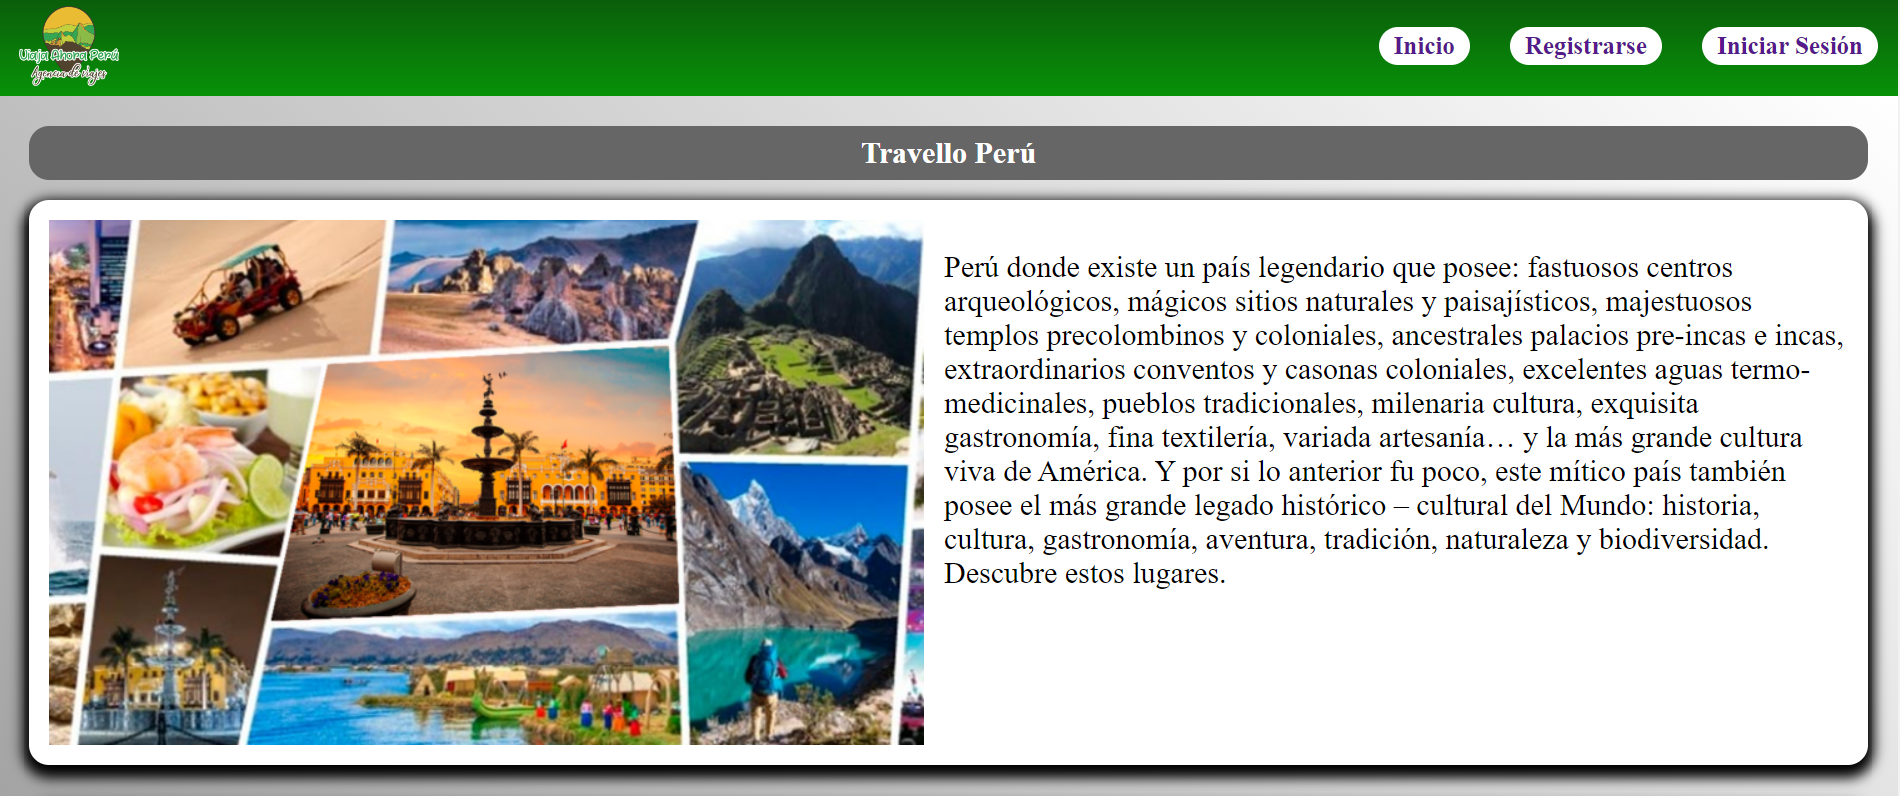
\includegraphics[width=16cm]{img/INICIO1.png}
            \\ \\
            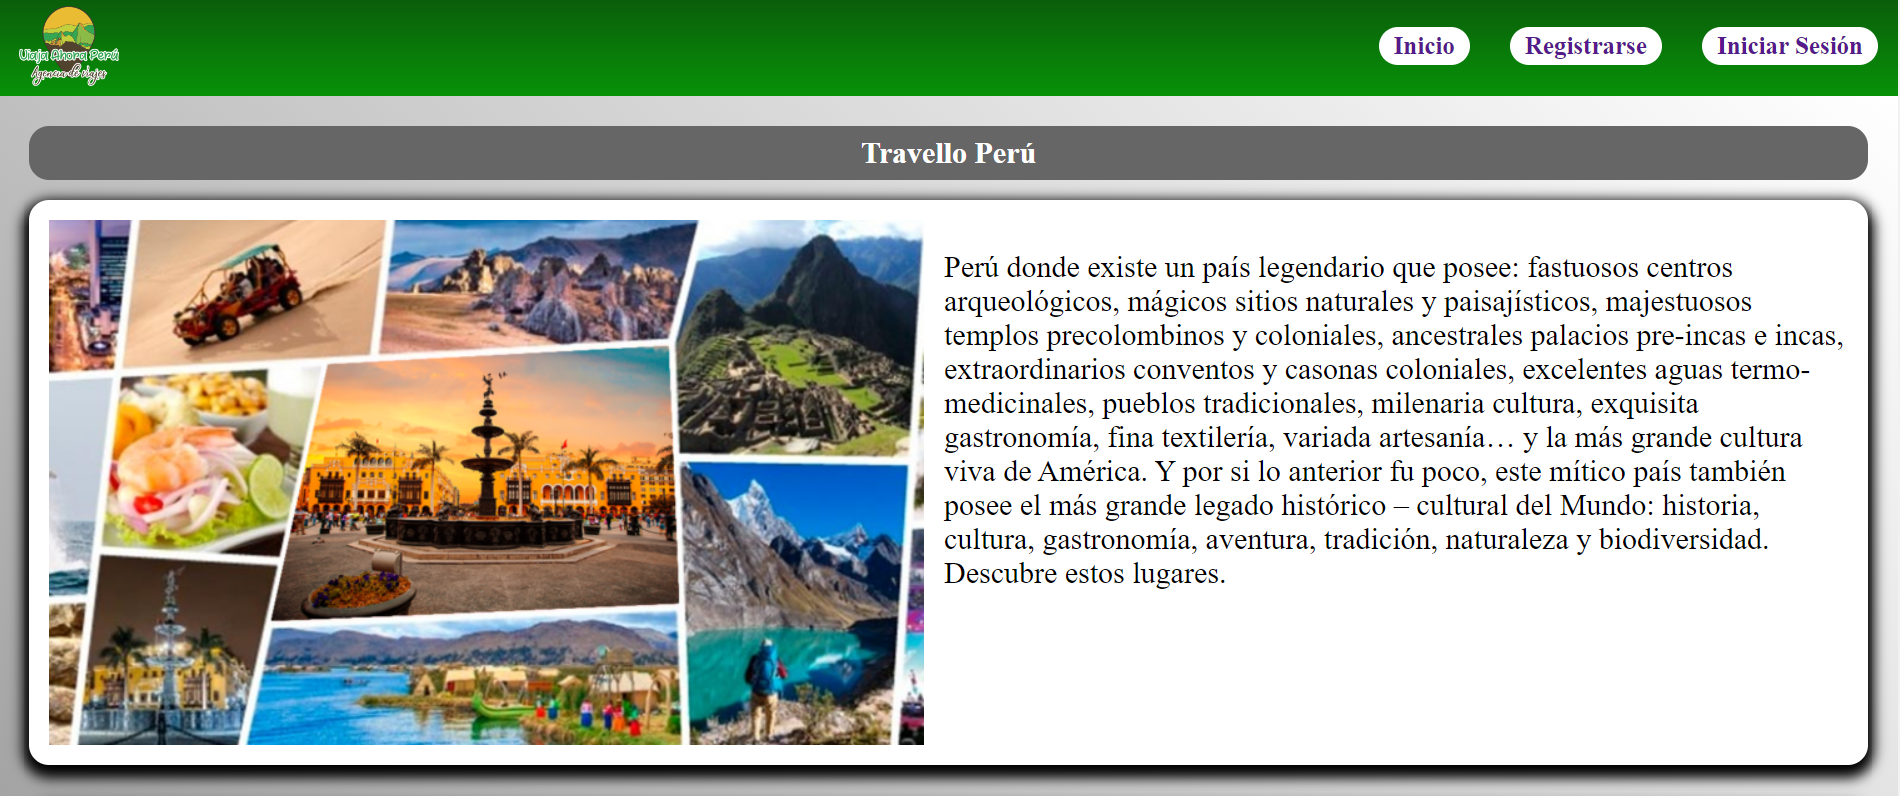
\includegraphics[width=16cm]{img/INICIO1.png}
            \\ \\
            Ahora nos registraremos.
            \\ \\
            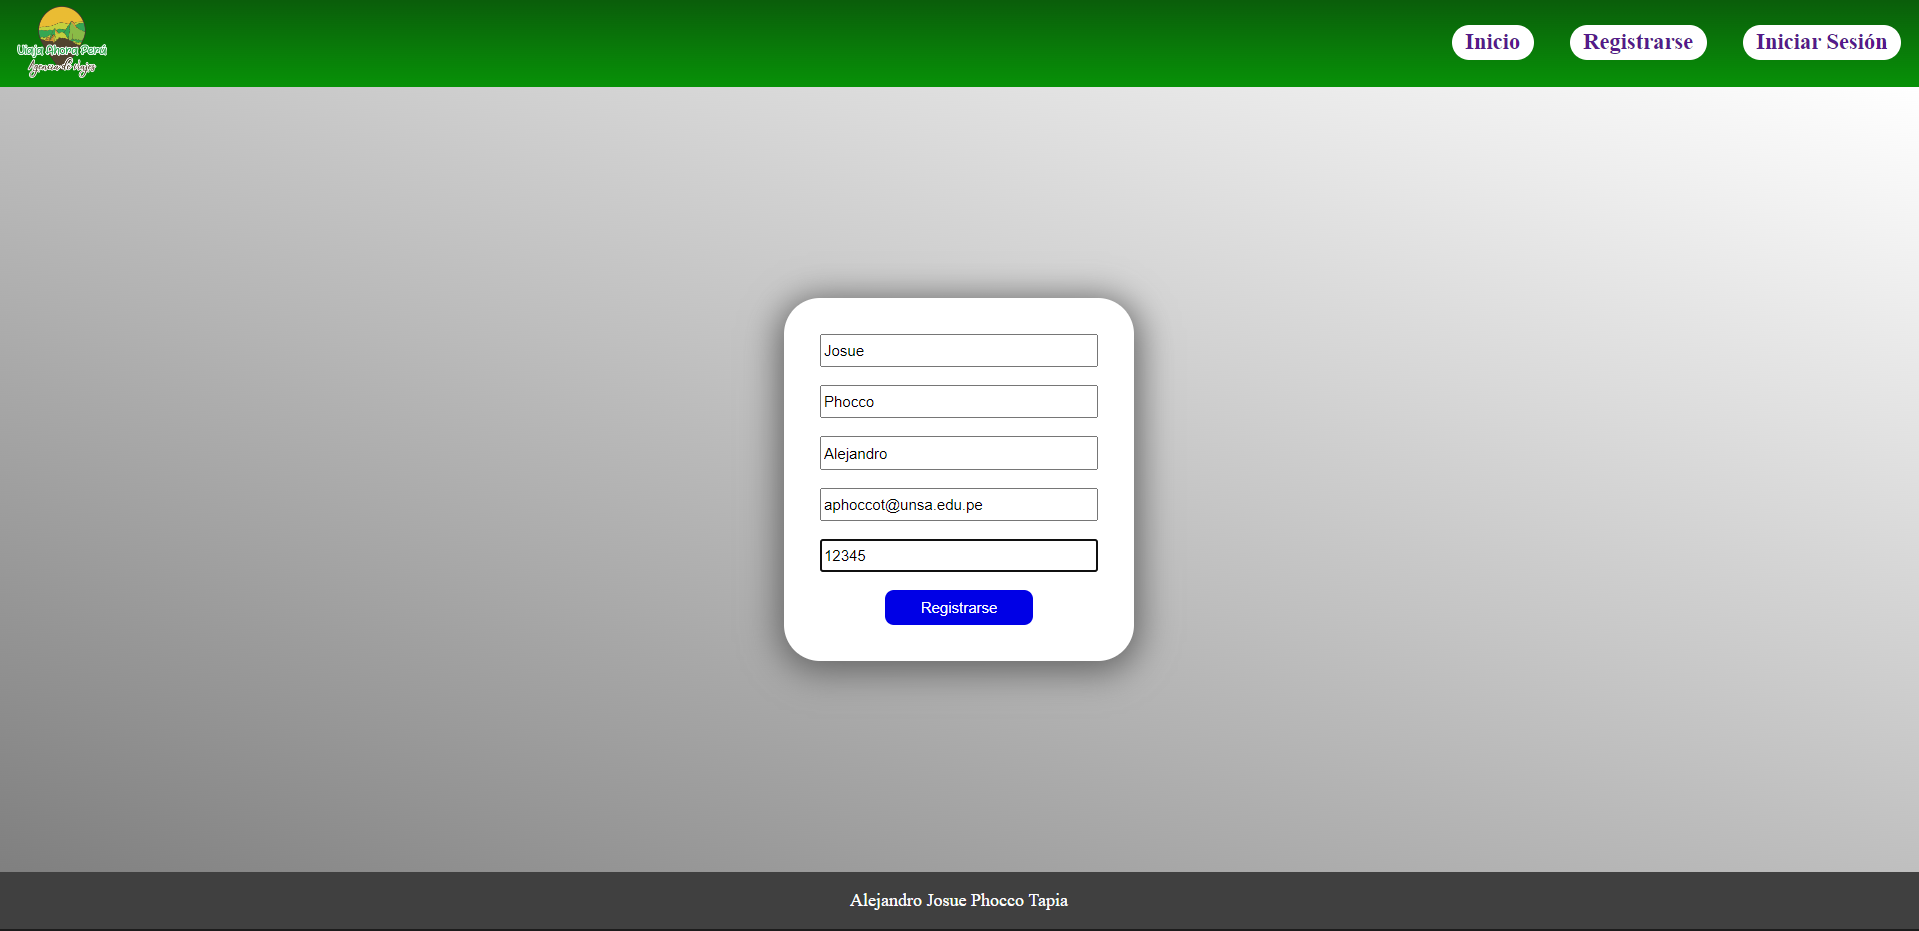
\includegraphics[width=16cm]{img/REGISTRARSE.png}
            \\ \\
            Ahora iniciaremos sesion con el usuario creado.
            \\ \\
            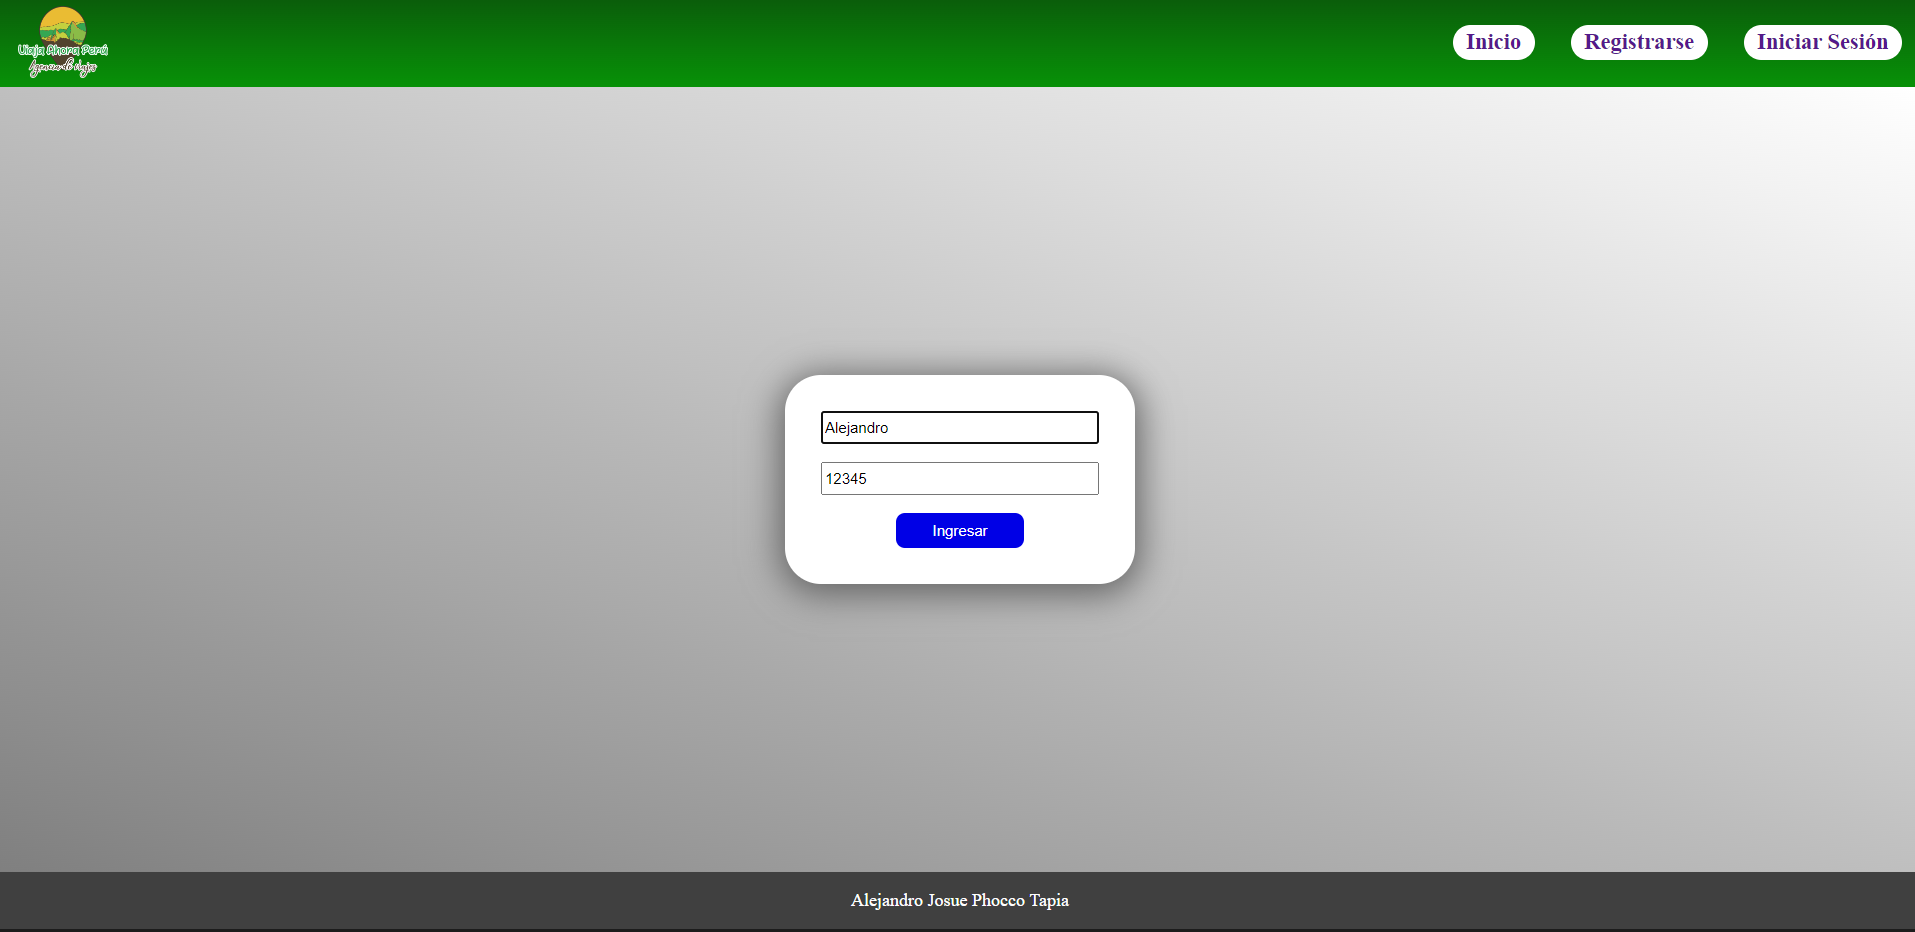
\includegraphics[width=16cm]{img/LOGIN.png}
            \\ \\
            Veremos que ahora la barra de navegacion cambia
            \\ \\
            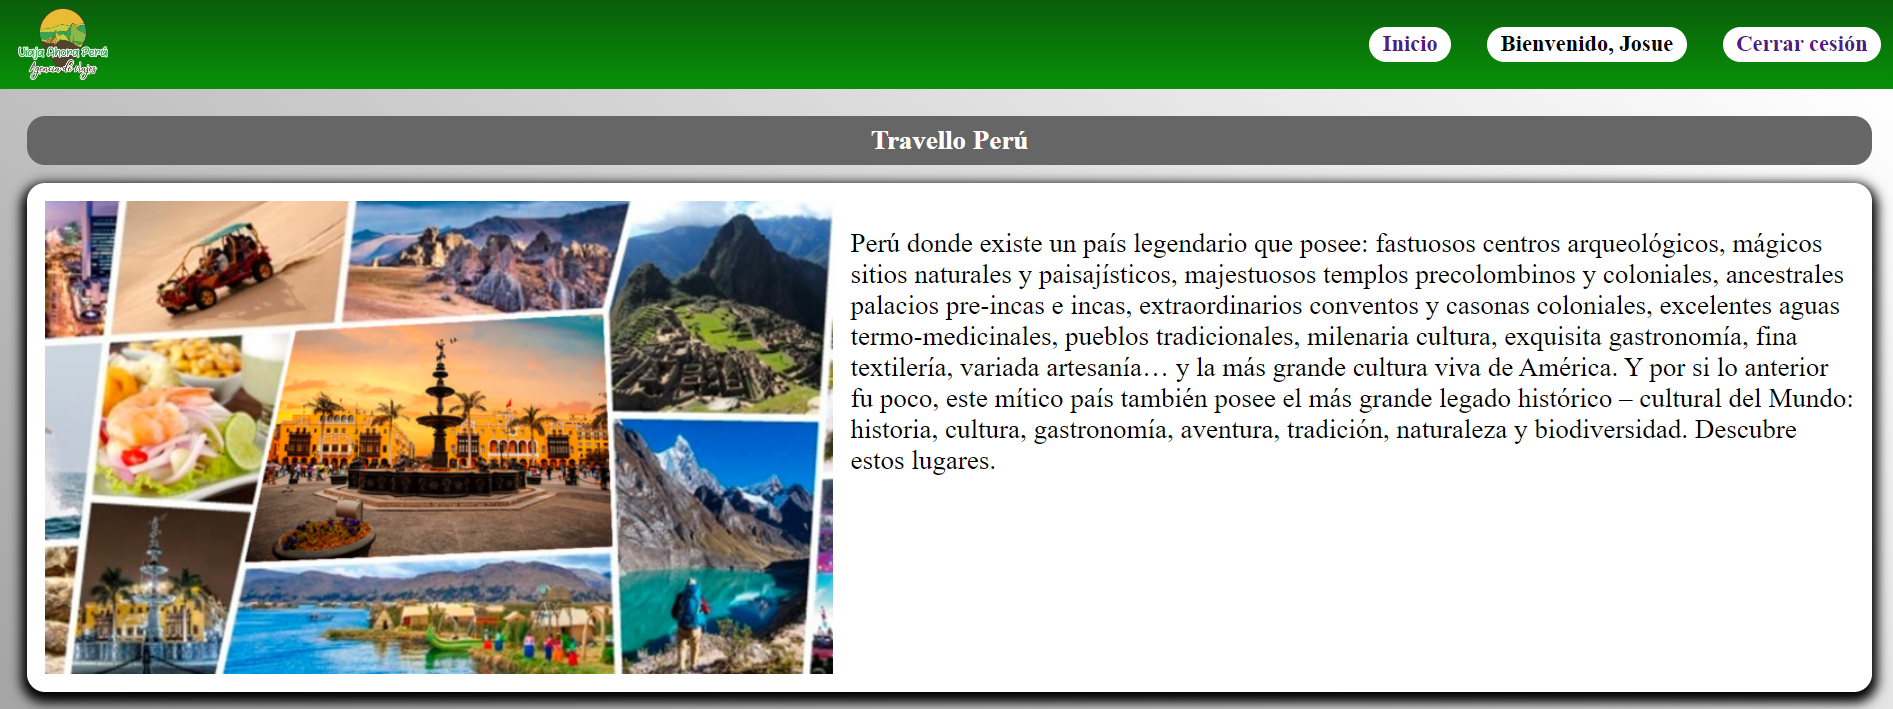
\includegraphics[width=16cm]{img/BARRA.png}
            \\ \\
            Ahora si entramos, a un destino observamos que tiene un mensaje especial si este tiene una oferta
            \\ \\
            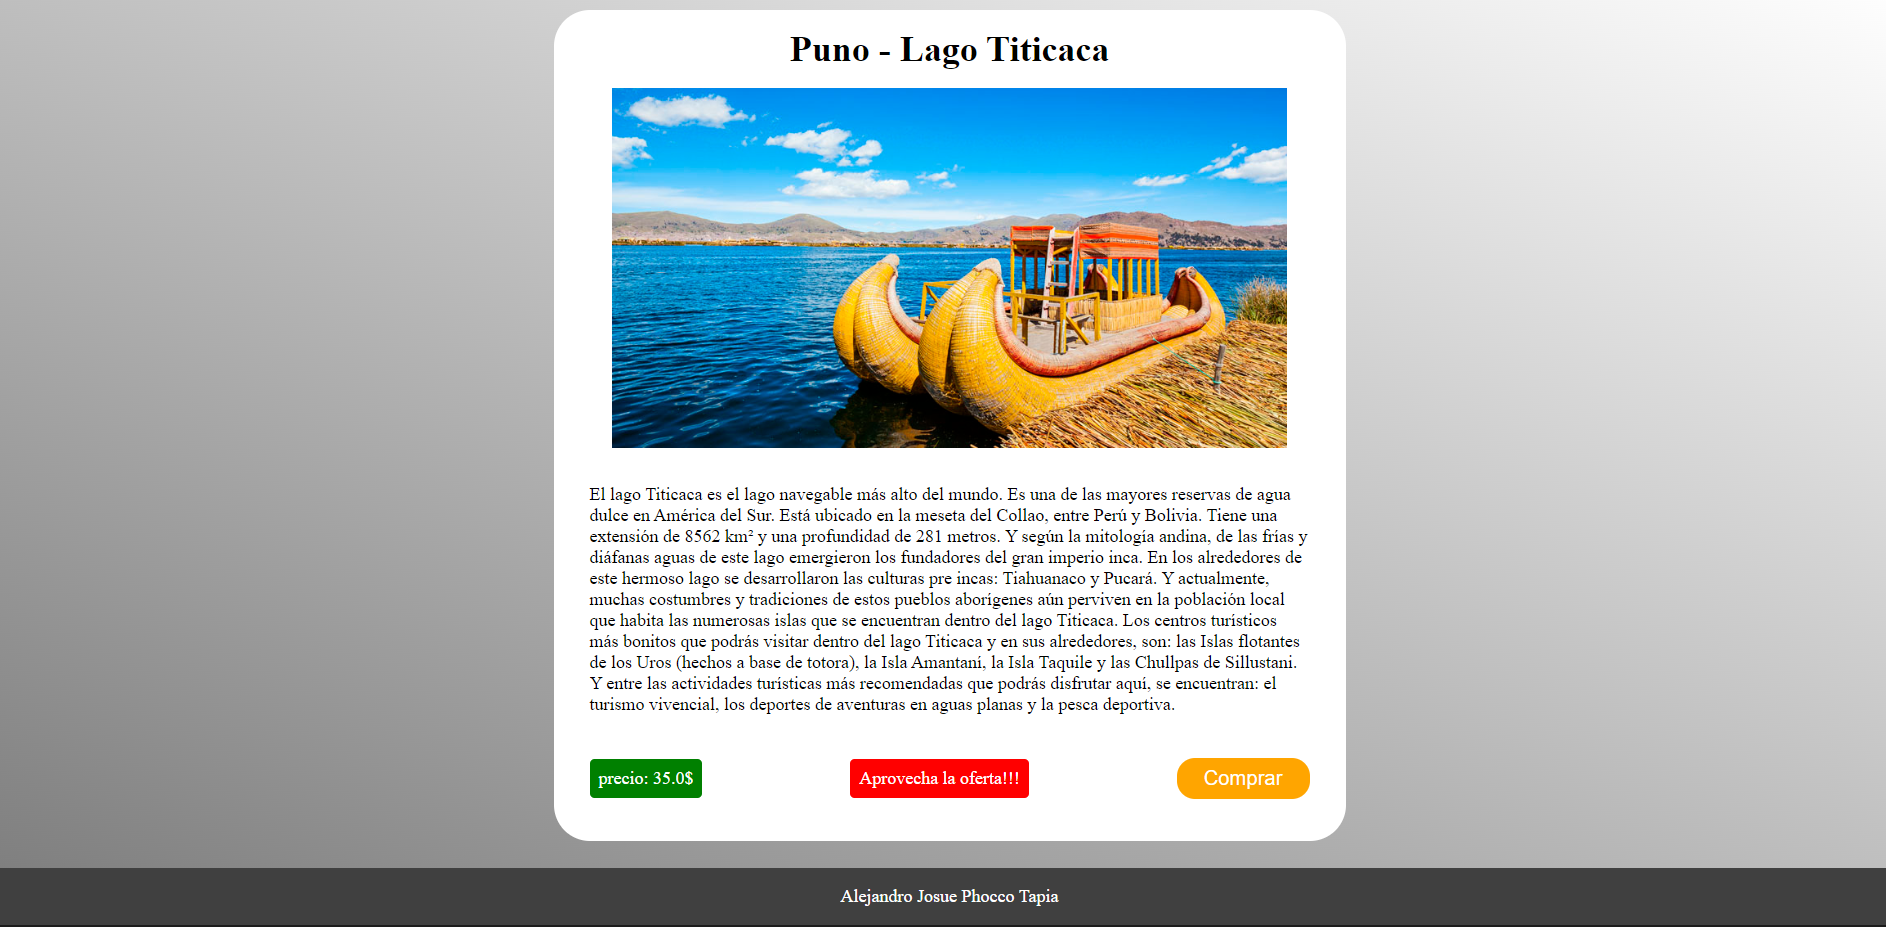
\includegraphics[width=16cm]{img/DESTINO.png}
            \\ \\
            Cuando presionamos cerrar sesion, veremos que la barra vuelve a su estado inicial.
            \\ \\
            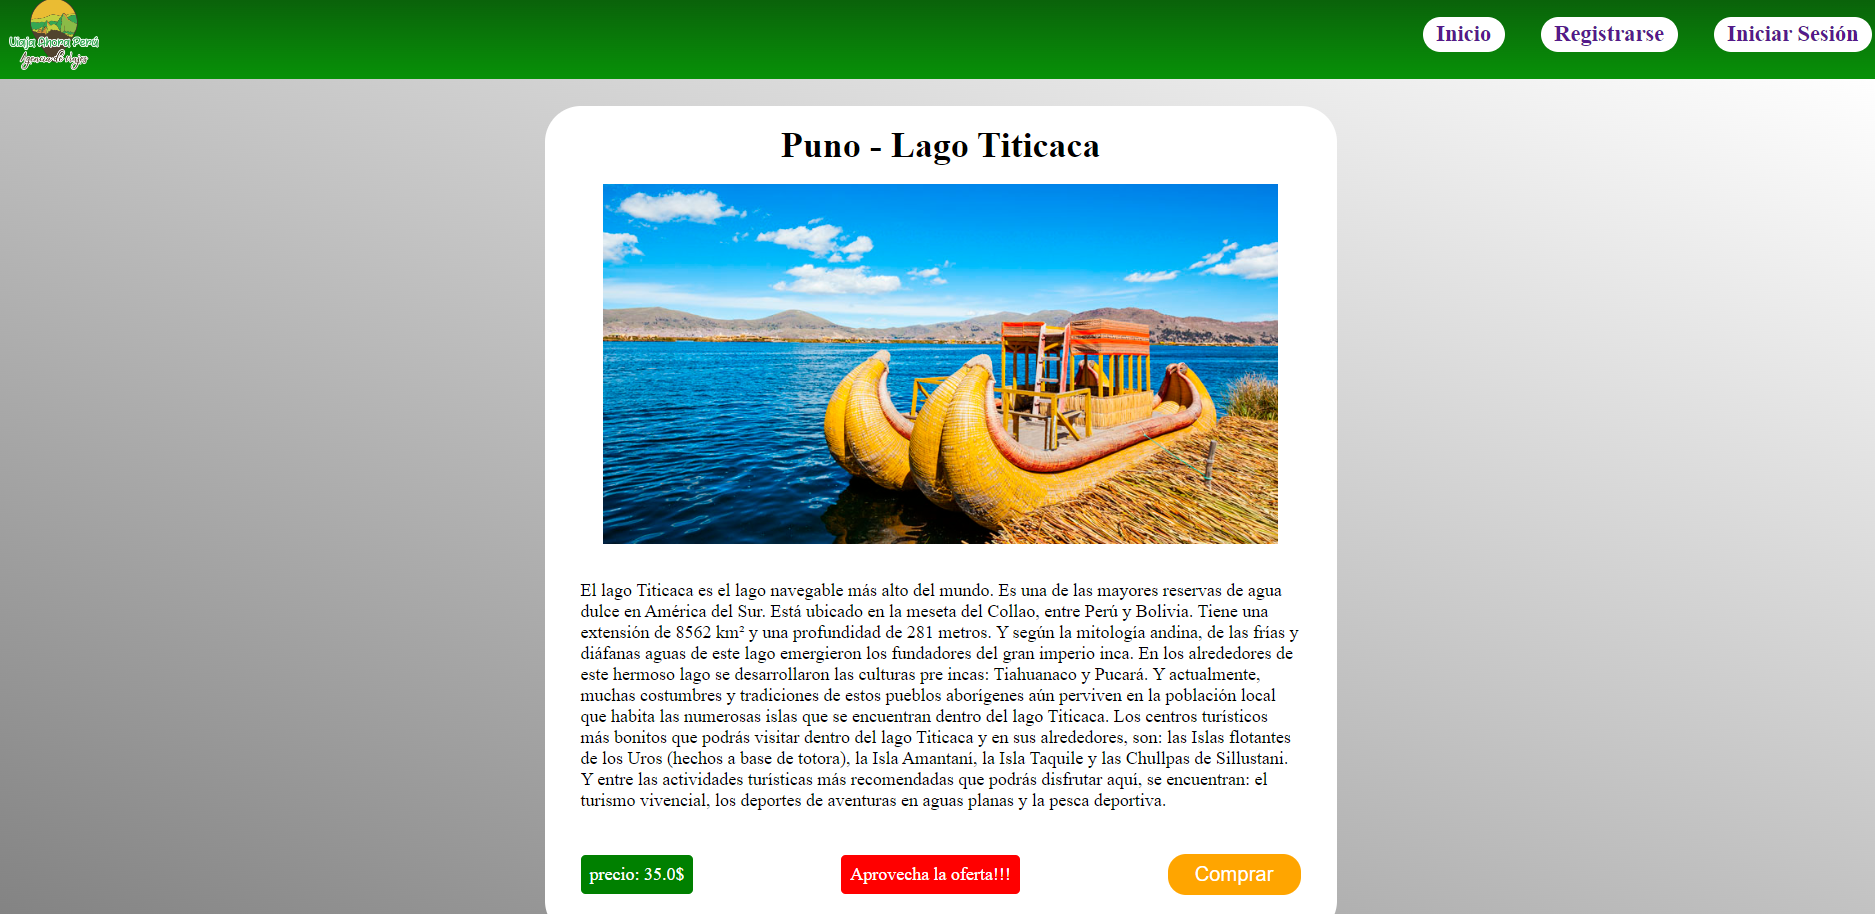
\includegraphics[width=16cm]{img/LOGOUT.png}
            \\ \\
            Observamos que todos los destinos estan guardados en la base de datos. Lo observamos a traves de la vista de administrador.
            \\ \\
            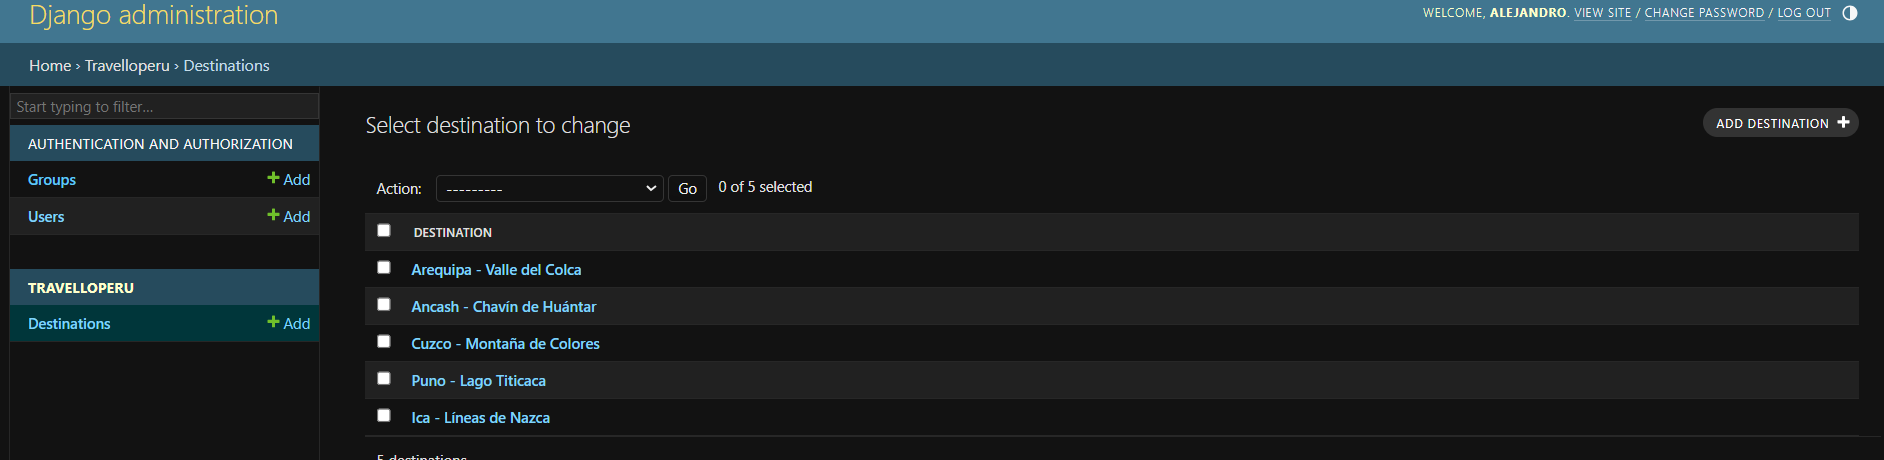
\includegraphics[width=16cm]{img/DESTINOSADMIN.png}
            \\ \\
            Por ultimo veremos tambien que el usuario que creamos se guardo en la base de datos.
            \\ \\
            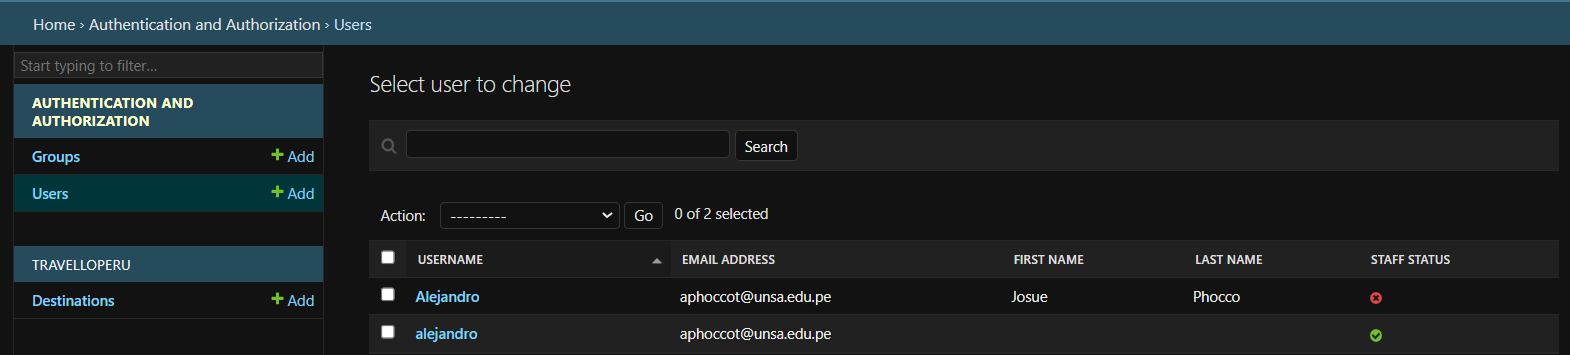
\includegraphics[width=16cm]{img/USERADMIN.png}
            
            
            
            Link donde esta alojado el video (FlipGrid):\newline
            GRUPO: \url{https://flip.com/groups/14644257/topics/36969916/responses} \\
            VIDEO ESPECIFICO: \url{https://flip.com/s/oX6doXAhZpyQ}
        
    \section{Cuestionario}
	- Sin cuestionario -	
 \newpage
    \section{Conclusiones}
	\begin{itemize}
		\item El uso de Django, como framework para trabajar tanto backend y frontend, es extremadamente util. Sus sistemas de plantillas, vistas, modelos y urls son muy utiles a la hora de enfocarse en trabajar enfocandonos en el producto, sin tener que preocuparnos por la seguridad o configuraciones del servidor. Por todo esto es muy beneficioso aprender a usar Django. 
	\end{itemize}	
\clearpage

    
    \section{Referencias}
        \begin{itemize}	
            \item \url{https://www.w3schools.com/python/python_reference.asp}
            \item \url{ https://docs.python.org/3/tutorial/}
            \item \url{https://docs.djangoproject.com/en/4.0/}
            \item \url{https://www.youtube.com/watch?v=M4NIs4BM1dk}
            \item \url{https://pip.pypa.io/en/latest/user_guide/}
            \item \url{https://www.youtube.com/watch?v=OTmQOjsl0eg}
        \end{itemize}	
	
%\clearpage
%\bibliographystyle{apalike}
%\bibliographystyle{IEEEtranN}
%\bibliography{bibliography}
			
\end{document}